%	paper.tex	Toby Searle
%	Last modified: Mon  7 Apr 18:12:55 2014
%	using jfm template

\NeedsTeXFormat{LaTeX2e}

\documentclass{jfm}

\usepackage{graphicx}
\usepackage{natbib}
%%%%%%%%%%%Added to template:
\usepackage{caption, subcaption, mathtools} % add my own packages
\graphicspath{ {./images/} }
\newcommand\Wi{\mbox{\textit{Wi}}}
\newcommand{\dt}[1]{\frac{d #1}{d t}} %time deriv
\newcommand{\dy}[1]{\frac{\partial #1}{\partial y}}
\newcommand{\me}{\mathrm{e}}
%%%%%%%%%%%%%%%

% See if the author has AMS Euler fonts installed: If they have, attempt
% to use the 'upmath' package to provide upright math.
\ifCUPmtlplainloaded \else
  \checkfont{eurm10}
  \iffontfound
    \IfFileExists{upmath.sty}
      {\typeout{^^JFound AMS Euler Roman fonts on the system,
                   using the 'upmath' package.^^J}%
       \usepackage{upmath}}
      {\typeout{^^JFound AMS Euler Roman fonts on the system, but you
                   dont seem to have the}%
       \typeout{'upmath' package installed. JFM.cls can take advantage
                 of these fonts,^^Jif you use 'upmath' package.^^J}%
       \providecommand\upi{\pi}%
      }
  \else
    \providecommand\upi{\pi}%
  \fi
\fi

% See if the author has AMS symbol fonts installed: If they have, attempt
% to use the 'amssymb' package to provide the AMS symbol characters.

\ifCUPmtlplainloaded \else
  \checkfont{msam10}
  \iffontfound
    \IfFileExists{amssymb.sty}
      {\typeout{^^JFound AMS Symbol fonts on the system, using the
                'amssymb' package.^^J}%
       \usepackage{amssymb}%
       \let\le=\leqslant  \let\leq=\leqslant
       \let\ge=\geqslant  \let\geq=\geqslant
      }{}
  \fi
\fi

% See if the author has the AMS 'amsbsy' package installed: If they have,
% use it to provide better bold math support (with \boldsymbol).

\ifCUPmtlplainloaded \else
  \IfFileExists{amsbsy.sty}
    {\typeout{^^JFound the 'amsbsy' package on the system, using it.^^J}%
     \usepackage{amsbsy}}
    {\providecommand\boldsymbol[1]{\mbox{\boldmath $##1$}}}
\fi

%%% Example macros (some are not used in this sample file) %%%

% For units of measure
\newcommand\dynpercm{\nobreak\mbox{$\;$dyn\,cm$^{-1}$}}
\newcommand\cmpermin{\nobreak\mbox{$\;$cm\,min$^{-1}$}}

% Various bold symbols
\providecommand\bnabla{\boldsymbol{\nabla}}
\providecommand\bcdot{\boldsymbol{\cdot}}
\newcommand\biS{\boldsymbol{S}}
\newcommand\etb{\boldsymbol{\eta}}

% For multiletter symbols
\newcommand\Real{\mbox{Re}} % cf plain TeX's \Re and Reynolds number
\newcommand\Imag{\mbox{Im}} % cf plain TeX's \Im
\newcommand\Rey{\mbox{\textit{Re}}}  % Reynolds number
\newcommand\Pran{\mbox{\textit{Pr}}} % Prandtl number, cf TeX's \Pr product
\newcommand\Pen{\mbox{\textit{Pe}}}  % Peclet number
\newcommand\Ai{\mbox{Ai}}            % Airy function
\newcommand\Bi{\mbox{Bi}}            % Airy function

% For sans serif characters:
% The following macros are setup in JFM.cls for sans-serif fonts in text
% and math.  If you use these macros in your article, the required fonts
% will be substitued when you article is typeset by the typesetter.
%
% \textsfi, \mathsfi   : sans-serif slanted
% \textsfb, \mathsfb   : sans-serif bold
% \textsfbi, \mathsfbi : sans-serif bold slanted (doesnt exist in CM fonts)
%
% For san-serif roman use \textsf and \mathsf as normal.
%
\newcommand\ssC{\mathsf{C}}    % for sans serif C
\newcommand\sfsP{\mathsfi{P}}  % for sans serif sloping P
\newcommand\slsQ{\mathsfbi{Q}} % for sans serif bold-sloping Q

% Hat position
\newcommand\hatp{\skew3\hat{p}}      % p with hat
\newcommand\hatR{\skew3\hat{R}}      % R with hat
\newcommand\hatRR{\skew3\hat{\hatR}} % R with 2 hats
\newcommand\doubletildesigma{\skew2\tilde{\skew2\tilde{\Sigma}}}
%       italic Sigma with double tilde

% array strut to make delimiters come out right size both ends
\newsavebox{\astrutbox}
\sbox{\astrutbox}{\rule[-5pt]{0pt}{20pt}}
\newcommand{\astrut}{\usebox{\astrutbox}}

\newcommand\GaPQ{\ensuremath{G_a(P,Q)}}
\newcommand\GsPQ{\ensuremath{G_s(P,Q)}}
\newcommand\p{\ensuremath{\partial}}
\newcommand\tti{\ensuremath{\rightarrow\infty}}
\newcommand\kgd{\ensuremath{k\gamma d}}
\newcommand\shalf{\ensuremath{{\scriptstyle\frac{1}{2}}}}
\newcommand\sh{\ensuremath{^{\shalf}}}
\newcommand\smh{\ensuremath{^{-\shalf}}}
\newcommand\squart{\ensuremath{{\textstyle\frac{1}{4}}}}
\newcommand\thalf{\ensuremath{{\textstyle\frac{1}{2}}}}
\newcommand\Gat{\ensuremath{\widetilde{G_a}}}
\newcommand\ttz{\ensuremath{\rightarrow 0}}
\newcommand\ndq{\ensuremath{\frac{\mbox{$\partial$}}{\mbox{$\partial$} n_q}}}
\newcommand\sumjm{\ensuremath{\sum_{j=1}^{M}}}
\newcommand\pvi{\ensuremath{\int_0^{\infty}%
  \mskip \ifCUPmtlplainloaded -30mu\else -33mu\fi -\quad}}

\newcommand\etal{\mbox{\textit{et al.}}}
\newcommand\etc{etc.\ }
\newcommand\eg{e.g.\ }


\newtheorem{lemma}{Lemma}
\newtheorem{corollary}{Corollary}

\title[Purely elastic self sustaining process]{Purely elastic self sustaining process}

\author[T. W. Searle and A. N. Morozov]%
{T. W. Searle$^1$ and A. N. Morozov$^1$%
  \thanks{Email address for correspondence: jfm@damtp.cam.ac.uk},\ns
}

% NOTE: A full address must be provided: department, university/institution, town/city, zipcode/postcode, country.
\affiliation{$^1$SUPA, School of Physics and Astronomy, University of Edinburgh, Mayfield Road,
Edinburgh, EH9 3JZ, UK\\[\affilskip]
}

\pubyear{2013}
\volume{650}
\pagerange{119--126}
% Do not enter received and revised dates. These will be entered by the editorial office.
\date{?; revised ?; accepted ?. - To be entered by editorial office}
%\setcounter{page}{1}
\begin{document}

\maketitle

\begin{abstract}
  Abstract goes here. Abstract goes here. Viscoelastic Kelvin-Helmholtz instability. 
\end{abstract}

\begin{keywords}
Authors should not enter keywords on the manuscript, as these must be chosen by the author during the online submission process and will then be added during the typesetting process (see http://journals.cambridge.org/data/\linebreak[3]relatedlink/jfm-\linebreak[3]keywords.pdf for the full list)
\end{keywords}

\section{Introduction}

\section{Methods}

\subsection{Streaky profile}

We use a Chebyshev-Fourier decomposition, with Chebyshev polynomials in the wall-normal (y) direction and Fourier modes in the spanwise (z) direction. We then solve for the velocity in the streamwise (x) direction, subject to forcing in the y and z directions, via a Newton-Raphson iteration of the governing Navier-Stokes and Oldroyd-B equations,
\begin{align}
    \Rey \left[ \dt{\mathbf{v}} + \mathbf{v} \cdot \nabla  \mathbf{v} \right] &= - \nabla p + \beta \nabla^{2} \mathbf{v} + \frac{1-\beta}{Wi} \nabla \cdot \mathbf{\tau} \label{eq:Navier-Stokes}\\
    \nabla \cdot \mathbf{v} &= 0 \label{eq:incompressibility}\\
    \dot{\tau}/Wi + \overset{\nabla}\tau &= \left(\nabla \mathbf{v}\right)^{T} + \nabla{\mathbf{v}}\label{eq:Oldroyd-B}
\end{align}
where $\Rey$ is the Reynold's number, $\Wi$ is the Weissenberg number, $\nabla$ is the gradient operator, $\nabla^{2}$ is the Laplacian and $ \overset{\nabla}\tau$ is the upper convected derivative of the stress tensor. In order to decompose the system onto the computational grid, we take a Fourier and Chebyshev transform of the variables,
\begin{equation}
    \check{G}(y,z) = \sum_{n=-N}^{N} \sum_{m=0}^{M+1} G_{m,n} \me{i\gamma z} T_{m}(y) \label{eq:decomp}
\end{equation}
where $g$ stands for any of the base profile variables ($U,V,W,\boldmath{\tau}_{ij}$) in the problem and $T_{m}(y)$ is the \textit{m}th Chebyshev polynomial of the first kind.

Given that the base profile is independent of the streamise direction and time, we reduce the Navier-Stokes and Oldroyd-B equations and then solve them using a simple Newton-Rhaphson iteration for the base Streamwise velocity $U$. The system is driven by the standard no-slip boundary conditions on the streamwise velocity at the walls,
\begin{align}
    U(\pm 1) = 1 \\
\end{align}
and forcing terms introduced via fixing of the wall-normal and spanwise base profile velocities,
\begin{align}
    V(y,z) &= V_0 \hat{v}(y) cos(\gamma z) \\
    W(y,z) &= \frac{V_0}{\gamma} \dy{\hat{v}} sin(\gamma z) 
\end{align}
Where,
\begin{equation}
    \hat{v}(y) = \frac{\cos(py)}{\cos(p)} - \frac{\cosh(\gamma y)}{cosh(\gamma)} 
\end {equation}
$p$ is given by solutions to $p\tan p + \gamma \tanh \gamma = 0$ and governs the number of rolls in the wall-normal direction. These velocities are a guess for the rolls derived from the lowest order eigenmode of the operator $\nabla^{4}$, precisely the same rolls used in \cite{Waleffe97}. This provides us with the streaky profile shown below.

\subsection{Linear Stability Analysis}

Having obtained the full base profile of the problem, we then performed a linear stability analysis, to look for instabilities that might produce waviness in the streaks. These wavy instabilities are responsible for sustaining the exact coherent state in the Newtonian version of the process.

We decompose the disturbance velocities in a similar way to above (equation \ref{eq:decomp}), but include streamwise dependence
\begin{equation}
    \check{g}(x,y,z,t) = \sum_{n=-N}^{N} \sum_{m=0}^{M+1} g_{m,n}(k_{x}) \me{i(k_{x} x + \gamma z)} T_{m}(y) \me{i\lambda t}\label{eq:decomp_disturbances}
\end{equation}
where $g$ can be any of the disturbance variables ($u,v,w,p,\boldmath{\tau}_{ij}$). To increase the numerical stability of the problem, we use free slip boundary conditions on the disturbance velocities, $\dy{w}(\pm1) = v(\pm 1) = \dy{w}(\pm1) = 0$.

The linearised system of equations now gives an eigenvalue problem for the growth rate of the instability $\lambda$ at every streamwise wavenumber of the disturbance.

The solution to the eigenvalue problem provides spectra for which eigenmodes with positive growth rates are unstable.

\section{Results}

\subsection{Streaks}

After using the above Newton-Rhaphson method we obtain a streaky profile in the fluid. At high $\Rey$ we find streaks in the streamwise velocity similar to those in \cite{Waleffe1997}. However, as we decrease the Reynold's number for constant and large Weissenberg number, we find that the streaks in the streamwise velocity become less pronounced. This can be explained by considering that at low Reynold's number the fluid has a higher inertia, so it is more difficult for the lift up effect to produce streaks in the streamwise velocity. 

Although we do not see streaks in the streamwise velocity, we do see them in the first normal stress difference, $N_{1} = T_{xx} - T_{yy}$ (figure \ref{fig:pf_N1_map}). These streaks appear in much the same place as the streamwise velocity streaks appear in the Newtonian self-sustaining process. As noted earlier, instabilities in viscoelastic fluids are brought about by large changes in the first normal stress difference, since this brings about polymer stretching of the kind seen in the Weissenberg effect. It is important to note that the purely elastic 1st normal stress difference shows very large gradients near the wall, suggesting that resolving the instability in this base profile will be more difficult than in the Newtonian case.

%\begin{figure}
%    \showthe\columnwidth %use this to determine size of figures.
%    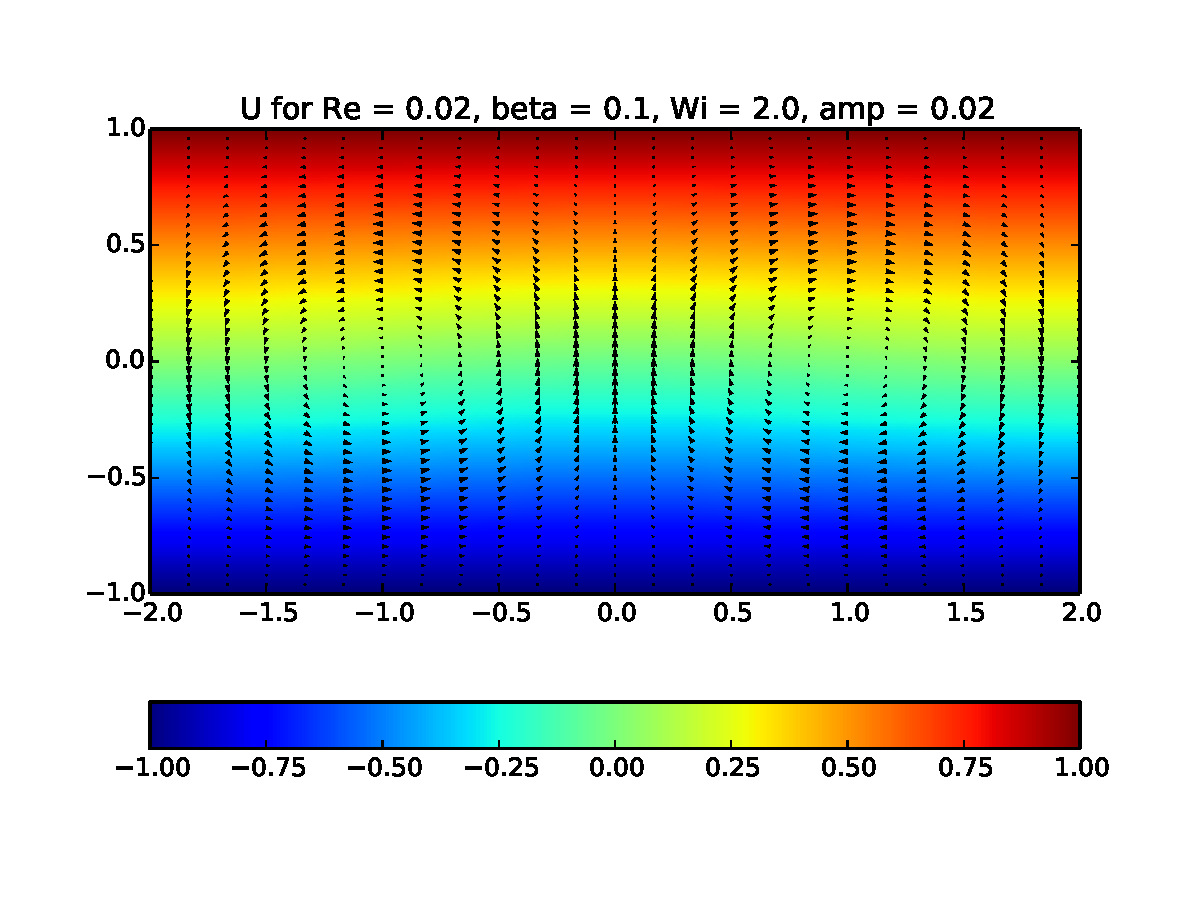
\includegraphics[width=\textwidth]{./figures/vel_map_Rey002_Wi2_amp002}
%    \caption{Streaky profile at $\Rey = 0.02$, $\Wi = 2.0$, amp=0.02. The heat map gives the streamwise velocity, U, whilst the arrows show direction the forcing from the rolls via the velocity in the wall-normal and spanwise directions.}
%    \label{fig:pf_vel_map}
%\end{figure}

\begin{figure}
    \centering
    \begin{subfigure}[b]{0.48\textwidth}
	\includegraphics[width=\textwidth]{./figures/vorticity_map_Re200_Wi2_amp002}
	\label{fig:pf_N1_map}
    \end{subfigure}
    ~
    \begin{subfigure}[b]{0.48\textwidth}
	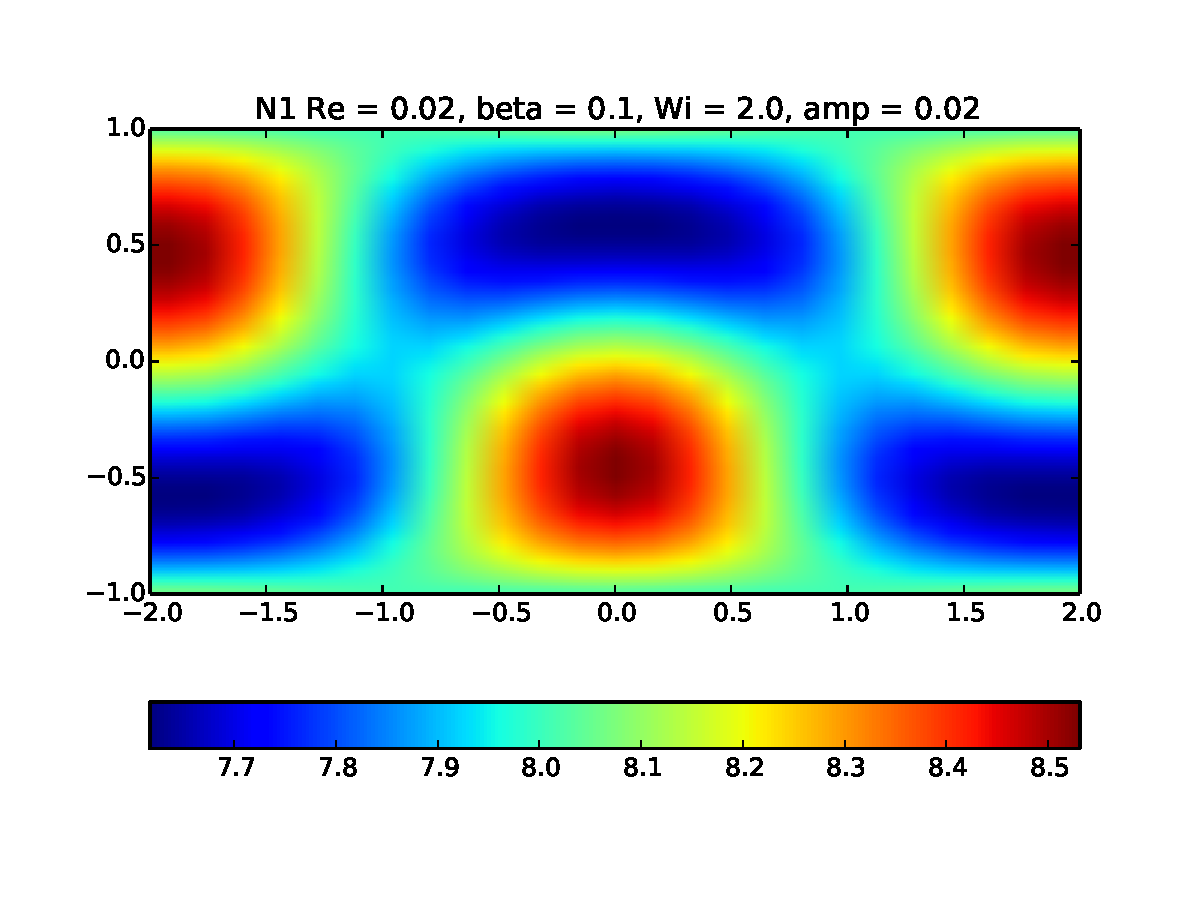
\includegraphics[width=\textwidth]{./figures/N1_map_Rey002_Wi2_amp002}
	\label{fig:pf_N1_map}
    \end{subfigure}
	\caption{a) The magnitude of the vorticity of the fluid at $\Rey = 200$, $\Wi = 2.0$, amp=0.02. b) The first normal stress difference in the polymeric fluid at $\Rey = 0.02$, $\Wi = 2$, amp=0.02. The Newtonian vorticity and purely elastic first normal stress difference have large gradients in similar regions. However, the first normal stress difference also shows large gradients next to the wall. }
\end{figure}

\subsection{Dispersion relations}

As the Reynold's number is decreased, we find that the base profile becomes more stable. The dispersion relation is reduced in height and moves to lower streamwise wavenumbers. By about $\Rey = 100$ the base profile has become completely stable. The Newtonian instability is no longer present at this Reynold's number. However, once the Reynolds number becomes negligible in comparison to the Weissenberg number, we begin to see a purely elastic instability arise at very low streamwise wavenumber \ref{fig:dispersions_varyRe}. This purely elastic instability is hugely amplified by further reductions in the Reynold's number.

\begin{figure}
%    \showthe\columnwidth %use this to determine size of figures.
    \centering
    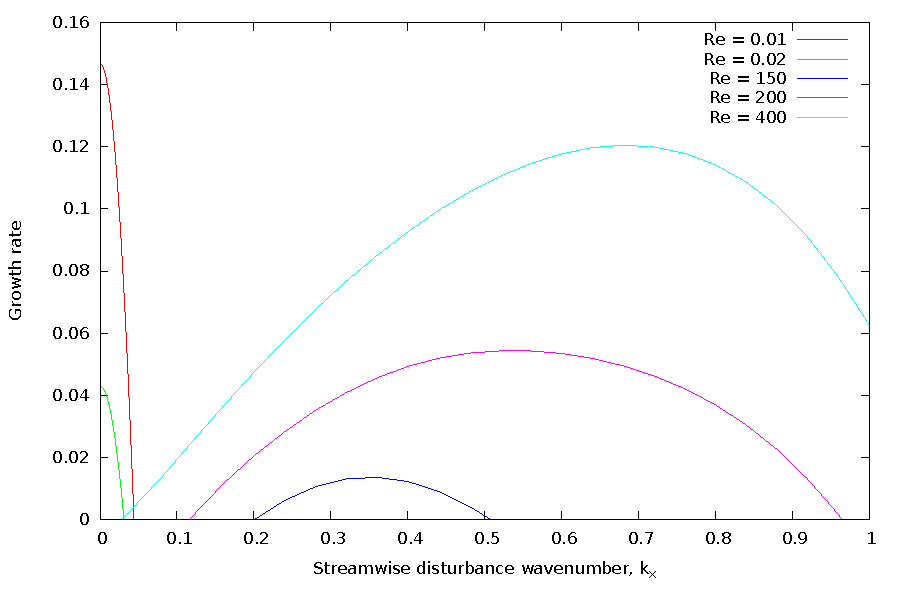
\includegraphics[width=\textwidth]{./figures/dispersions_varyRe}
    \caption{Dispersion relations as the Reynold's number is decreased at $\Wi = 2$, $\beta=0.1$ and amp = 0.02. A clear instability can be seen at low $k_{x}$ in the purely elastic regime.}
    \label{fig:dispersions_varyRe}
\end{figure}

We can further examine how the purely elastic instability changes with changing Weissenberg number. We find that it grows as the Weissenberg number increases, and saturates by around $\Wi ~ 20$. Doubling the amplitude of the rolls increases the width of the instablity by about a third and the height, 3 fold.  

\begin{figure}
%    \showthe\columnwidth %use this to determine size of figures.
    \centering
    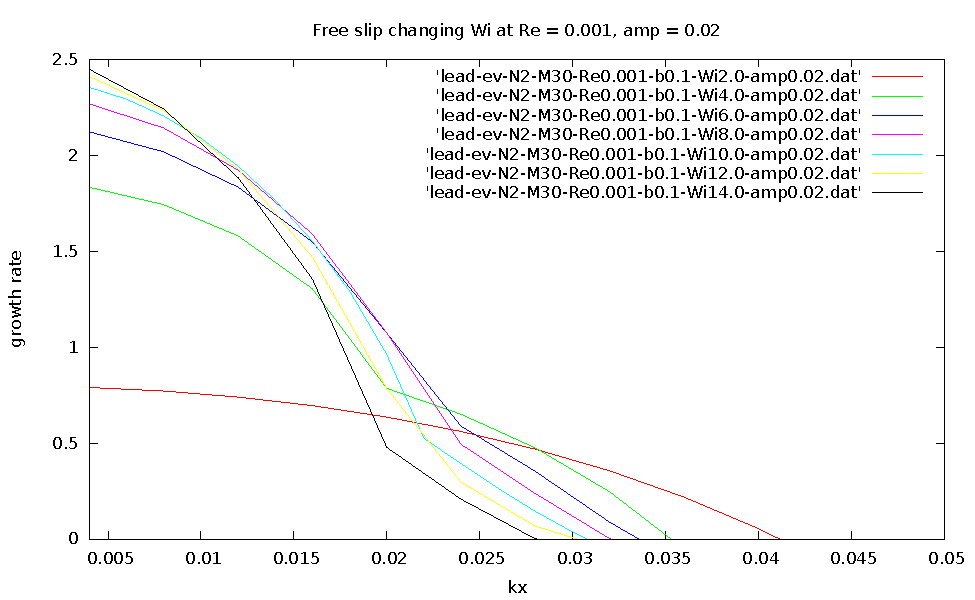
\includegraphics[width=\textwidth]{./figures/dispersions_varyWi}
    \caption{Dispersion relations as the $\Wi$ is decreased at $\Rey = 0.001$, $\beta=0.1$ and amp = 0.02. The instability grows and then saturates.}
    \label{fig:dispersions_varyWi}
\end{figure}

\subsection{eigenmodes}

In Fabian Waleffe's treatment of the Newtonian version of this self-sustaining process \cite{Waleffe1997}, he found that the feedback on the original rolls was provided by the eigenmode of the instability. The eigenmodes of the viscoelastic instability is quite different to that of the Newtonian instability. Although the components of the instability are large at the walls, the velocity is less important for the instability of the purely elastic fluid than the first normal stress difference. We find that $N_{1}$ is large away from the walls, another encouraging sign for a viscoelastic self-sustaining process (\ref{fig:eigenmode_visco}).

\begin{figure}
%    \showthe\columnwidth %use this to determine size of figures.
    \centering
    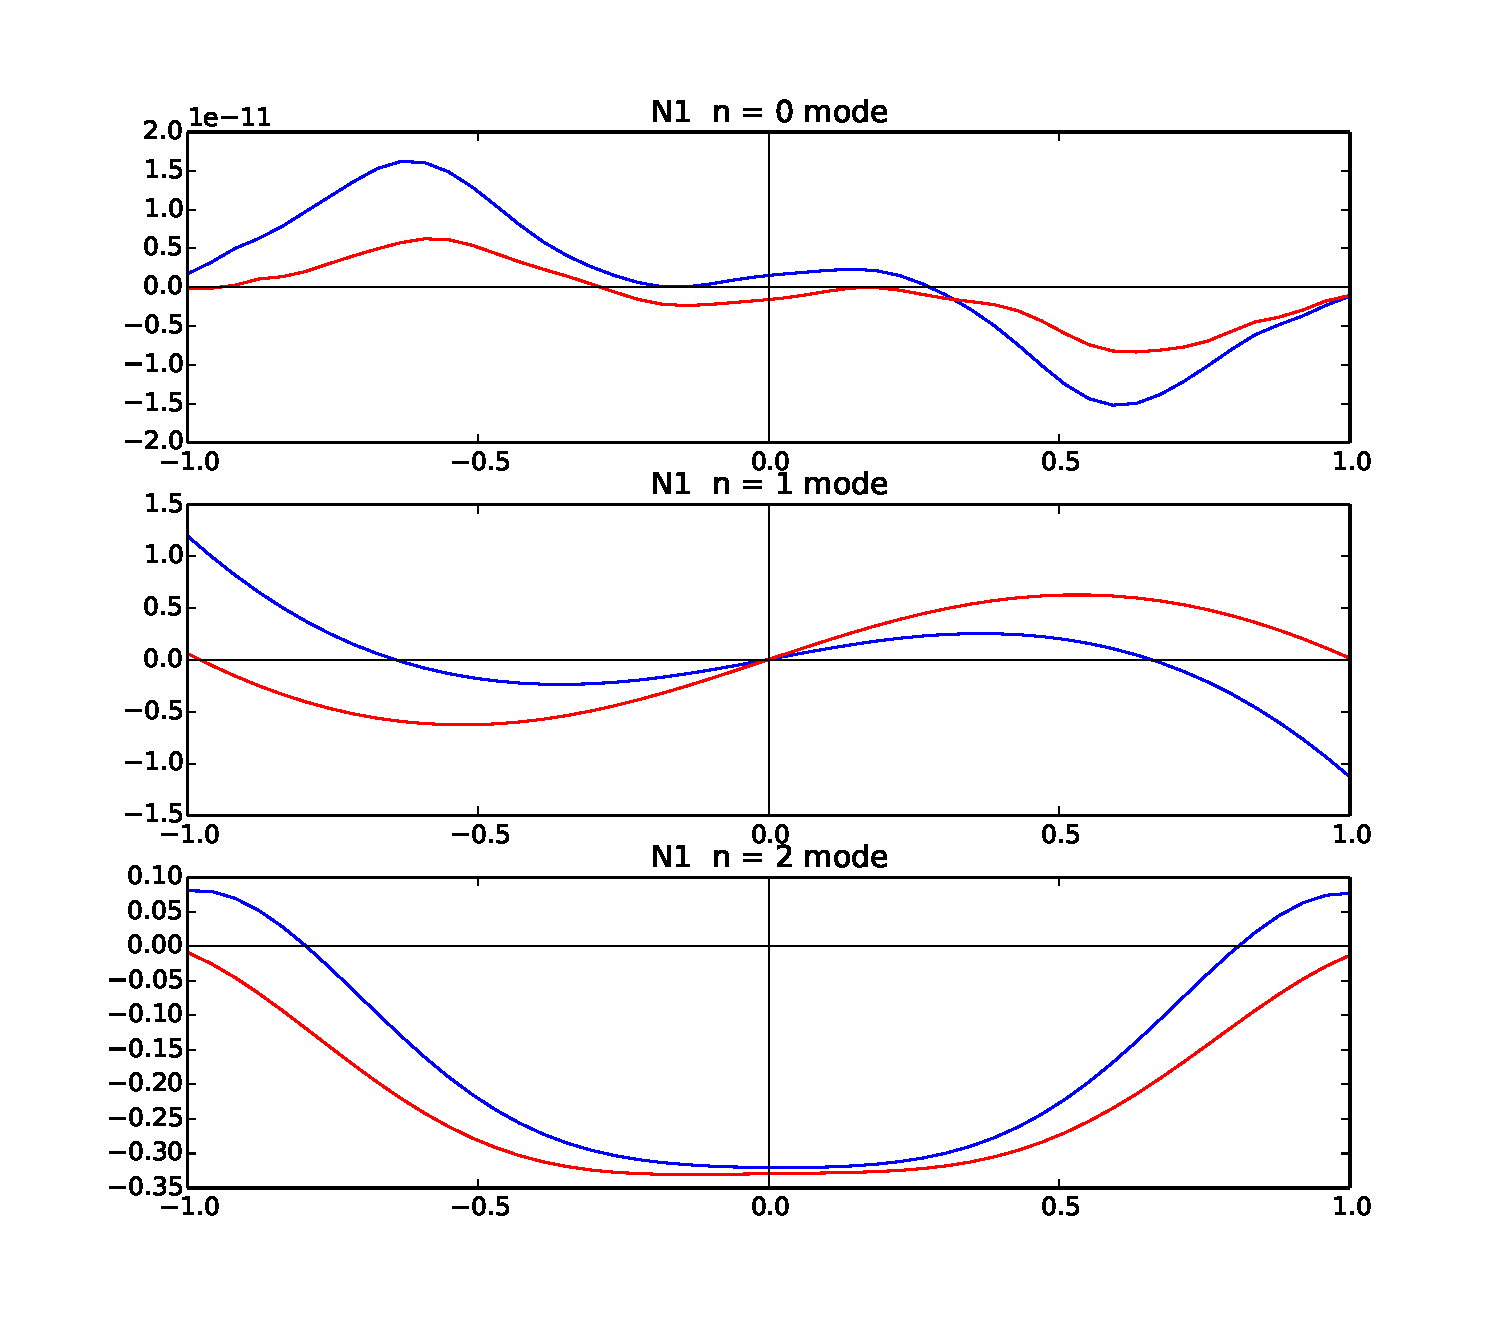
\includegraphics[width=\textwidth]{./figures/eigenmode_visco}
    \caption{Eigenmodes of the first normal stress difference of the viscoelastic instability at $\Wi = 2.0$, $\Rey = 0.02$, $\beta=0.1$, amp=0.02 and $k_x = 0.01$.}
    \label{fig:eigenmode_visco}
\end{figure}

\subsection{Cauchy boundary conditions}

\section{No slip case}

\section{Discussion}

\section{Conclusion}

\begin{figure}
%    \showthe\columnwidth %use this to determine size of figures.
    \centering
    
\includegraphics[width=0.7\textwidth]{./figures/robot}
    \caption{}
    \label{fig:KH_drag_reduction}
\end{figure}


\bibliographystyle{jfm}
% Note the spaces between the initials


\bibliography{KH_paper}

\end{document}
